For the algorithm in section~\ref{sec:data_and_algorithm} a few other methods will be used. As they are not the focus of this work we only give a short overview.

\section{Classification}
\label{subsec:classification}

In classification the objective is to find assignments between data points and categories. In our context we are interested in finding an assignment which closely matches some already categorized data. One simple approach to this problem is the k-nearest-neighbors algorithm.

For data that can be represented in $\mathbbm{R}^m$ and $l$ categories the pseudo code is shown in algorithm~\ref{alg:k_nearest_neighbors}.

\begin{algorithm}
	\caption{k Nearest Neighbors}\label{alg:k_nearest_neighbors}
	\begin{algorithmic}
		\Require data points $(p_i)_{i \in \mathbbm{N}} \in \mathbbm{R}^{m}$, categories $(c_i)_{i \in \mathbbm{N}} \in \{0, 1, ..., l\}$, point $x \in \mathbbm{R}^{m}$, $k \in \mathbbm{N}$
		\State Calculate the distance between each point $p_i$ and $x$
		\State Take the $k$ data points with the smallest distance to $x$
		\State Return the category that most of the $k$ points are assigned
	\end{algorithmic}
\end{algorithm}

Figure~\ref{fig:k_nearest_neighbors} shows a graphical representation of the algorithm for points in $\mathbbm{R}^2$ and $k=10$.

\begin{figure}
	\centering
	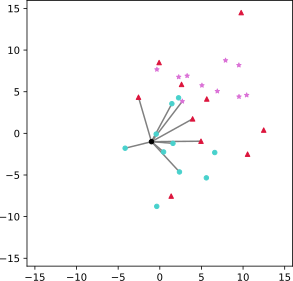
\includegraphics[width=\linewidth]{figs/k_nearest_neighbors}
	\caption{Data points in three categories are given. The black point is classified as a blue, circular point by the k-nearest-neighbors algorithm for $k=10$.}
	\label{fig:k_nearest_neighbors}
\end{figure}

This algorithm is slow for big datasets as for each point the distance to $x$ has to be calculated. One possibility to reduce calculation time is to partition space into smaller chunks. Then the loop only has to be over data points lying in the same or close chunks as the point we are interested in.

\section{Fourier Transformation}
\label{subsec:fourier_transformation}

[TODO]
